% Source: tex/chapters/ch05/07_テスト関連測度.tex
\subsection{テスト関連測度}
測度は、テスト目標が達成されたかを判断するために必要である。テスト技法は道具であり、測度はその道具が目的に役立っているかを判断する根拠である。測度は、テスト計画の最適化、進捗管理、品質分析、完了判断に使われる。

\begin{figure}[htbp]
\centering
\IfFileExists{assets/generated_figures/ch05/fig-ch05-11.png}{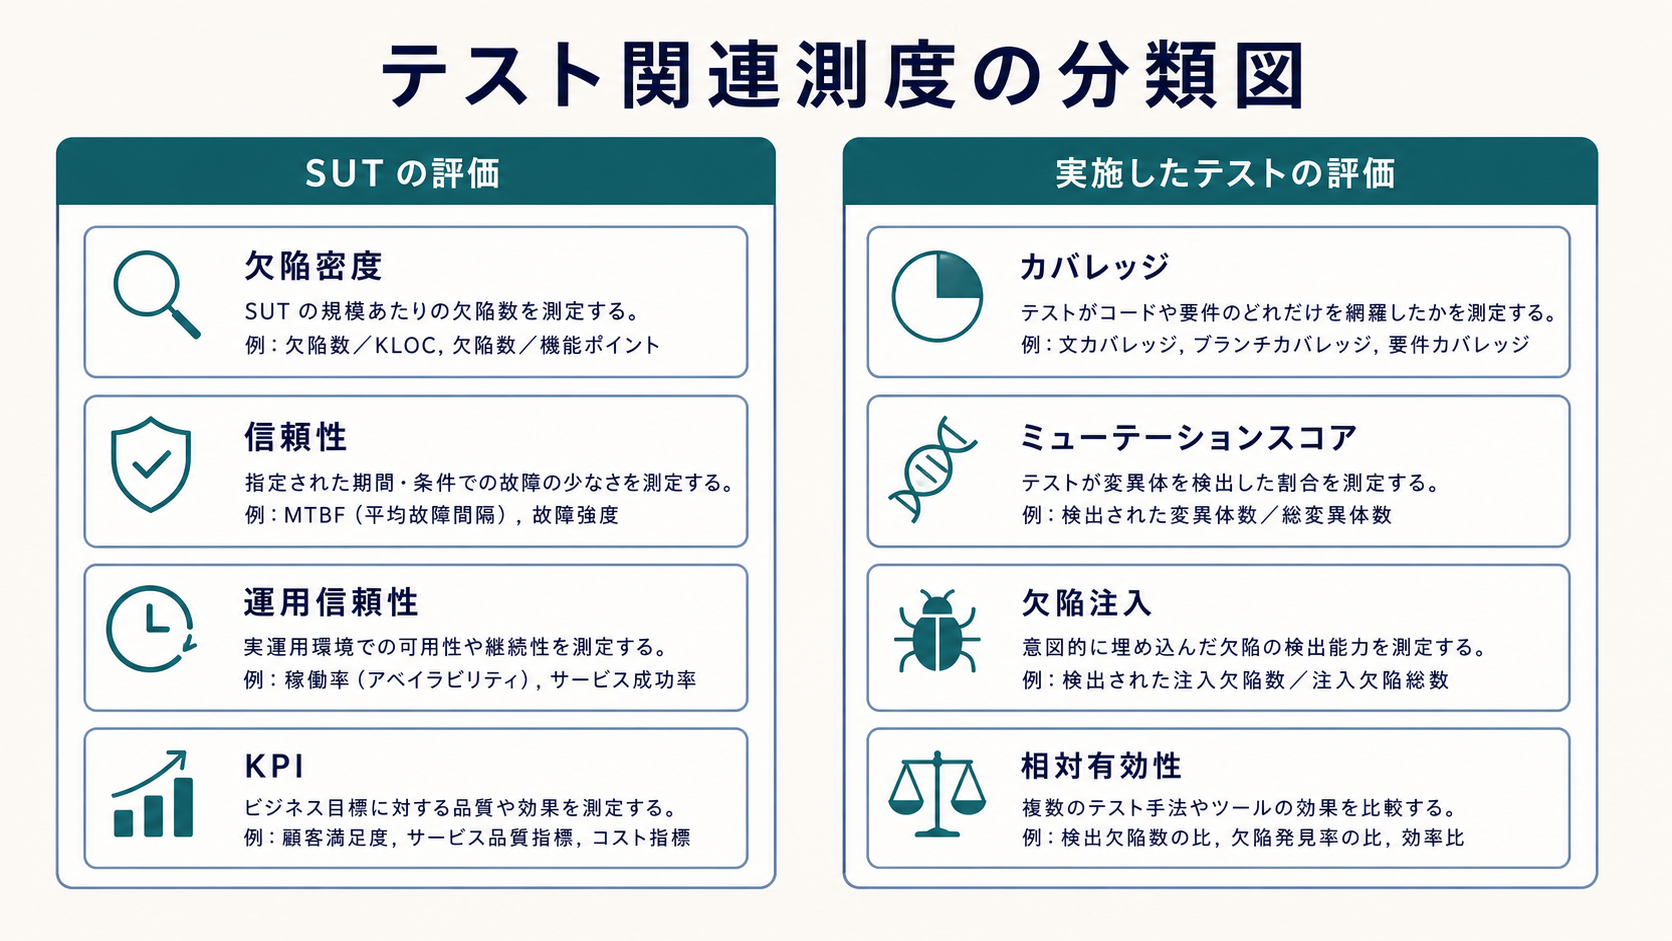
\includegraphics[width=0.96\linewidth]{assets/generated_figures/ch05/fig-ch05-11.png}}{\fbox{\parbox[c][48mm][c]{0.9\linewidth}{\centering 画像生成待ち\\テスト関連測度の分類図}}}
\caption{テスト関連測度の分類図}
\label{fig:ch05-11}
\end{figure}
